\documentclass[10pt,final,a4paper,oneside,onecolumn]{article}

%%==========================================================================
%% Packages
%%==========================================================================
\usepackage[a4paper,left=3.5cm,right=3.5cm,top=3cm,bottom=3cm]{geometry} %% change page layout; remove for IEEE paper format
\usepackage[T1]{fontenc}                        %% output font encoding for international characters (e.g., accented)
\usepackage[cmex10]{amsmath}                    %% math typesetting; consider using the [cmex10] option
\usepackage{amssymb}                            %% special (symbol) fonts for math typesetting
\usepackage{amsthm}                             %% theorem styles
\usepackage{dsfont}                             %% double stroke roman fonts: the real numbers R: $\mathds{R}$
\usepackage{mathrsfs}                           %% formal script fonts: the Laplace transform L: $\mathscr{L}$
\usepackage[pdftex]{graphicx}                   %% graphics control; use dvips for TeXify; use pdftex for PDFTeXify
\usepackage{array}                              %% array functionality (array, tabular)
\usepackage{upgreek}                            %% upright Greek letters; add the prefix 'up', e.g. \upphi
\usepackage{stfloats}                           %% improved handling of floats
\usepackage{multirow}                           %% cells spanning multiple rows in tables
%\usepackage{subfigure}                         %% subfigures and corresponding captions (for use with IEEEconf.cls)
\usepackage{subfig}                             %% subfigures (IEEEtran.cls: set caption=false)
\usepackage{fancyhdr}                           %% page headers and footers
\usepackage[official,left]{eurosym}             %% the euro symbol; command: \euro
\usepackage{appendix}                           %% appendix layout
\usepackage{xspace}                             %% add space after macro depending on context
\usepackage{verbatim}                           %% provides the comment environment
\usepackage[dutch,USenglish]{babel}             %% language support
\usepackage{wrapfig}                            %% wrapping text around figures
\usepackage{longtable}                          %% tables spanning multiple pages
\usepackage{pgfplots}                           %% support for TikZ figures (Matlab/Python)
\pgfplotsset{compat=1.14}						%% Run in backwards compatibility mode
\usepackage[breaklinks=true,hidelinks,          %% implement hyperlinks (dvips yields minor problems with breaklinks;
bookmarksnumbered=true]{hyperref}   %% IEEEtran: set bookmarks=false)
%\usepackage[hyphenbreaks]{breakurl}            %% allow line breaks in URLs (don't use with PDFTeX)
\usepackage[final]{pdfpages}                    %% Include other pdfs
\usepackage[capitalize]{cleveref}				%% Referensing to figures, equations, etc.
\usepackage{units}								%% Appropriate behavior of units
\usepackage[utf8]{inputenc}   				 	%% utf8 support (required for biblatex)
%\usepackage{csquotes}							%% Quoted texts are typeset according to rules of main language
%\usepackage[style=ieee,doi=false,isbn=false,url=false,date=year,minbibnames=15,maxbibnames=15,backend=biber]{biblatex}
%%\renewcommand*{\bibfont}{\footnotesize}		%% Use this for papers
%\setlength{\biblabelsep}{\labelsep}
%\bibliography{../../bib}
\usepackage{siunitx}

%%==========================================================================
%% Define reference stuff
%%==========================================================================
\crefname{figure}{Figure}{Figures}
\crefname{equation}{}{}

%%==========================================================================
%% Define header/title stuff
%%==========================================================================
\newcommand{\progressreportnumber}{36}
\renewcommand{\author}{Erwin de Gelder}
\renewcommand{\date}{January 28, 2021}
\renewcommand{\title}{Performance assessment of automated vehicles using real-world driving scenarios}

%%==========================================================================
%% Fancy headers and footers
%%==========================================================================
\pagestyle{fancy}                                       %% set page style
\fancyhf{}                                              %% clear all header & footer fields
\fancyhead[L]{Progress report \progressreportnumber}    %% define headers (LE: left field/even pages, etc.)
\fancyhead[R]{\author, \date}                           %% similar
\fancyfoot[C]{\thepage}                                 %% define footer

\begin{document}
	
\begin{center}
	\begin{tabular}{c}
		\title \\ \\
		\textbf{\huge Progress report \progressreportnumber} \\ \\
		\author \\ 
		\date
	\end{tabular}
\end{center}

\section{Previous meeting minutes}

\begin{itemize}
	\item We briefly discussed the plans for the paper on \emph{risk quantification}. Jan-Pieter mentioned that we should complement scenarios with ``domain knowledge'' for elements for which little to no data is available, such as rare events.
\end{itemize}

\section{Summary of work}

\begin{itemize}
	\item I worked on a paper called ``A Surrogate Safety Metric for Risk Evaluation''. The goal of the paper is to present a metric that can determine real-time the probability of a collision. The sections on the literature review and the method are finished. A review of these sections would be highly appreciated. The current version of the paper is attached to this report (pages 3 till 17).
	
	Once finished, my plan is to submit the paper to Accident Analysis \& Prevention (from Elsevier, impact factor is 3.655).
	
	\item I finished the experiments regarding a new method for generating test scenarios. Attached to this report, you can find the ``PowerPoint version'' of the paper I want to write (pages 18 till 30). If no major issues are raised, I will start with writing the paper.
	
	Once finished, my plan is to submit the paper to IEEE Transactions on Intelligent Transportation Systems (impact factor is 6.319).
	
	\item For the practical use of the scenario generation within TNO, a necessary element is the possibility to do conditional sampling. For example, we would like to sample ``cut-in scenarios'', such that the ego vehicle is driving at \SI{100}{\kilo\meter\per\hour}.
	While working on the new method for generating test scenarios, I realized that our current way of conditional sampling would not work. The current way of conditional sampling assumes that a part of the vector $x$ that we want to sample is fixed. E.g., that the first element of $x$ needs to be $100$. With the new method for generating test scenarios, the condition that, e.g., the ego vehicle is driving at \SI{100}{\kilo\meter\per\hour}, results in a linear constraint of the form
	\begin{equation}
		\label{eq:linear constraint}
		Ax = b.
	\end{equation}
	Luckily, it is still possible to perform conditional sampling, but I could not found a way to do so in literature. Therefore, I documented the method that I now use to perform the conditional sampling in case of a linear constraint like \cref{eq:linear constraint}.
	
	I described the method in a small report (see page 31-43). I discussed this work with Eric Cator (prof Applied Stochastics at TU Nijmegen). He thinks that it might be well suitable for an applied conference. Therefore, I was thinking of trying to submit it to Intelligent Vehicles Symposium (deadline: February 15). 
\end{itemize}

\section{Future plans}

In \cref{fig:planning}, the updated planning is shown. There are a few changes compared to the planning shown in the previous progress report:
\begin{itemize}
	\item I extended the time for the ``ontology'' paper. The paper has been submitted, so I am waiting for the reviewers' feedback.
	\item I added the conference paper on conditional sampling.
\end{itemize}

\begin{figure}[t]
	\centering
	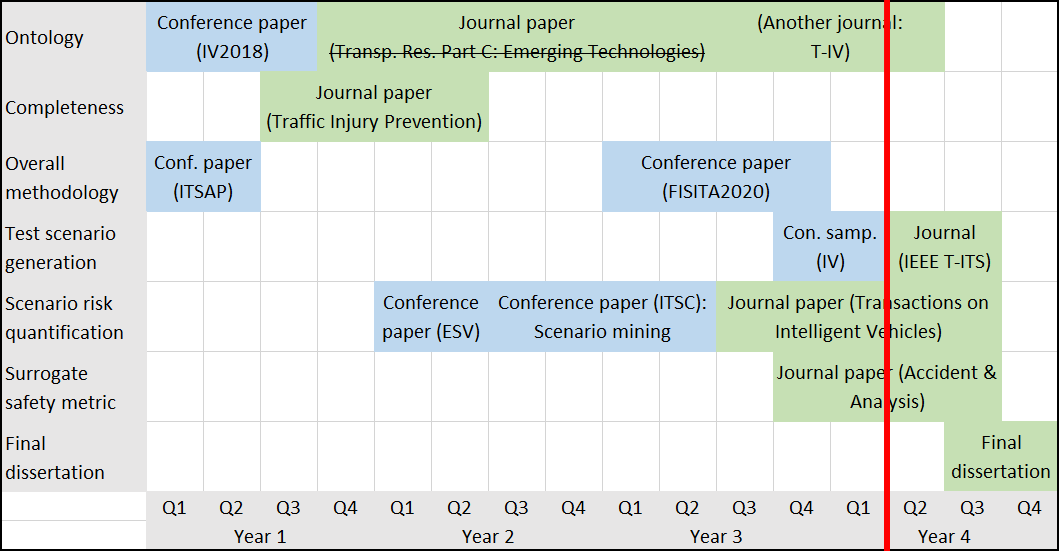
\includegraphics[width=\linewidth]{planning.png}
	\caption{Proposed planning at the time of this report. The red line indicated the time when writing this report.}
	\label{fig:planning}
\end{figure}

For the coming weeks, I want to focus on the following:
\begin{itemize}
	\item Rewrite the report on the conditional sampling, such that it is suitable for submission to the Intelligent Vehicle Symposium (extended deadline: February 1). In the introduction, I want to explain first that we use Kernel Density Estimation (KDE) to generation test scenarios for the assessment of automated vehicles (this is not new). The contribution of the paper is then on the sampling from these KDEs. 
	
	\item Start with writing for the paper for generation of test scenarios.
	
	\item Finish the draft of the paper on the \emph{surrogate safety metric}.
\end{itemize}


\section{Questions}

\begin{itemize}
	\item Given the tight deadline for the Intelligent Vehicles Symposium (February 15), I wonder if it is realistic to ask and process feedback. 
	\begin{itemize}
		\item Would this be a problem? 
		\item How about the authorship?
		\item Would it be useful to ask Eric Cator for feedback (which means that he becomes a co-author)? (My proposed answer: Yes)
	\end{itemize}
	
	\item Would it be possible to review Sections 2 and 3 of ``A Surrogate Safety Metric for Risk Evaluation'' (page 3-17)?
	
	\item Are there major issues/concerns related to ``Scenario Generation and Comparison for the Assessment of Automated Vehicles'' (page 18-30)? If not, I will start writing soon. 
\end{itemize}


%\printbibliography

\clearpage
\includepdf[pages=-,pagecommand={},width=\paperwidth]{../../"20201126 Risk Metric"/main.pdf}
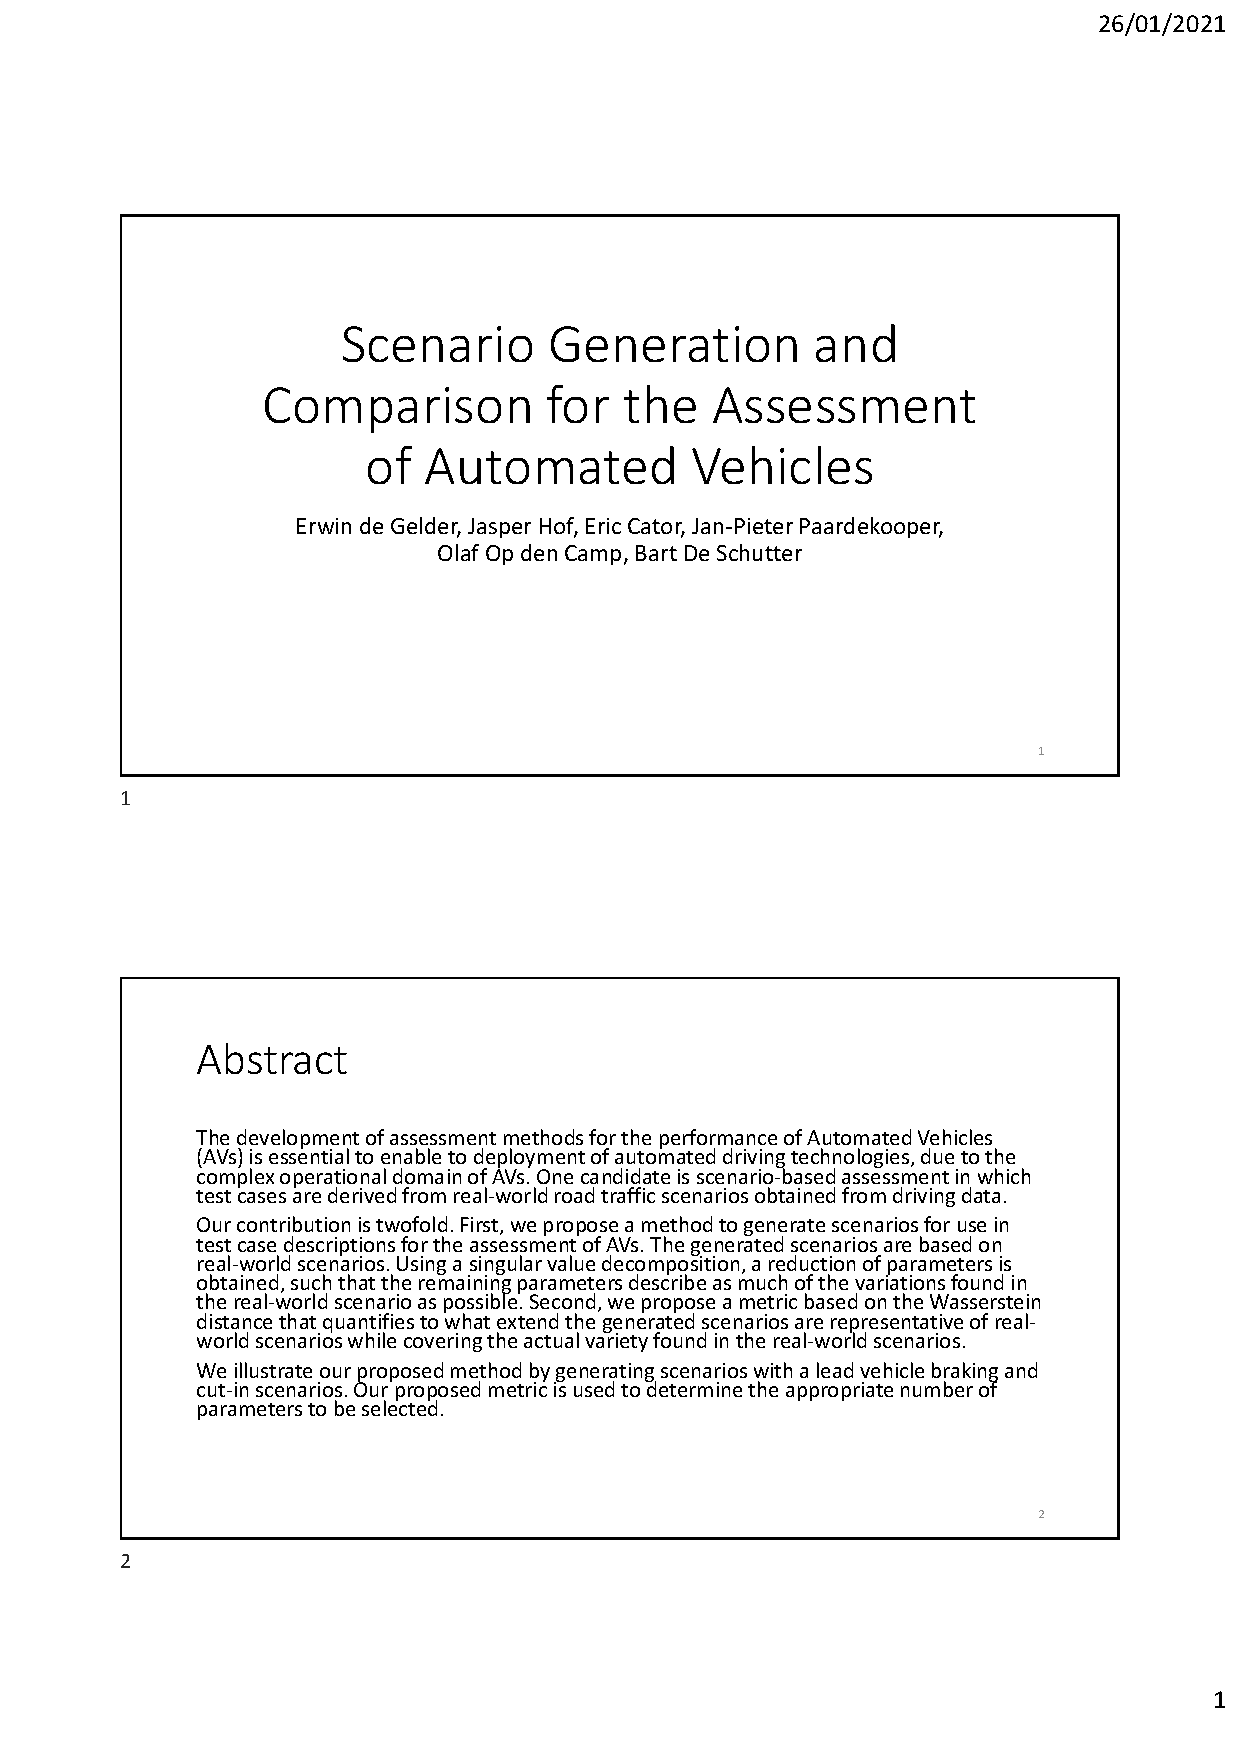
\includepdf[pages=-,pagecommand={},width=\paperwidth]{outline_tcg.pdf}
\includepdf[pages=-,pagecommand={},width=\paperwidth]{../../"20201221 Conditional Sampling"/conditional_sampling.pdf}

\end{document}